\chapter{Resultados}
\label{resultados}

\section{Dados Obtidos}
Os dados armazenados foram extraídos do banco de dados em um arquivo no formato CSV, \emph{Comma Separated Values} (Valores Separados por Vírgula), o arquivo apresenta as informações descritas na Seção \ref{experimento} e contém um total de 462.065 linhas. Na Figura \ref{fig:csv_example} são ilustradas as primeiras linhas do arquivo CSV. A partir do arquivo CSV, foram gerados onze novos arquivos, um para cada dispositivo Tx, contendo o identificador do pacote, o horário da transmissão e quais tentativas de transmissão foram bem sucedidas. Na Figura \ref{fig:second_csv_example} é ilustrado um desses arquivos, em que o número ``1'' significa uma tentativa de transmissão bem sucedida e o número ``0'' significa que não foi recebida a mensagem com a modulação daquele identificador.


\begin{figure}[h]
      \centering
      \caption{Dados do experimento.}
      \begin{subfigure}{.8\textwidth}
            \centering
            \caption{Exemplo das Colunas do Arquivo CSV.}
            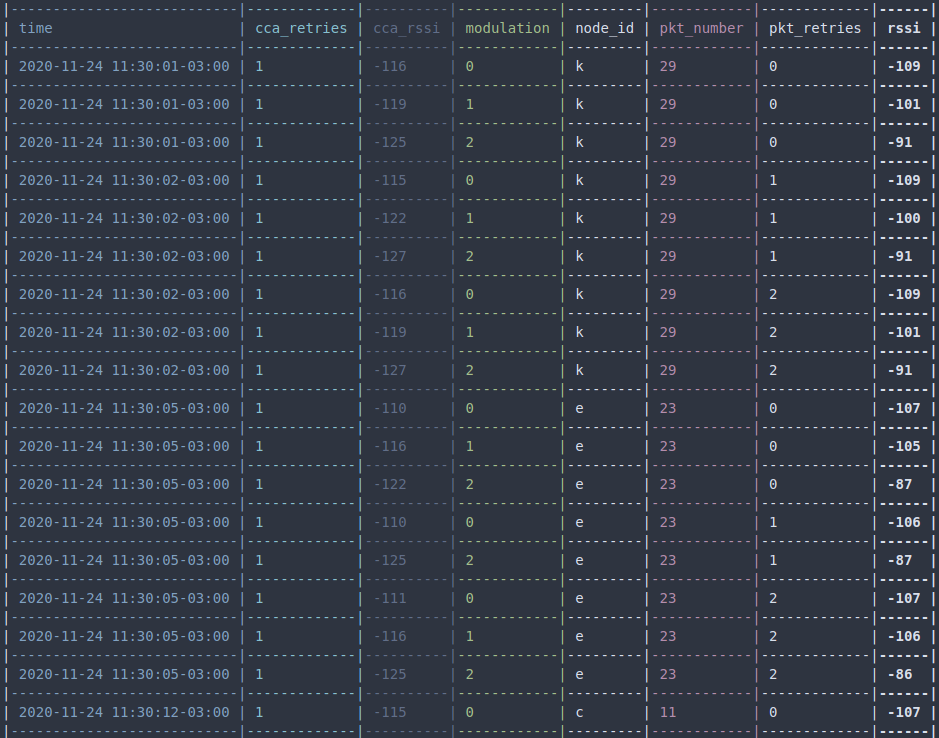
\includegraphics[width=\textwidth]{./sections/textual/chapters/images/csv_example.png}
            \label{fig:csv_example}
      \end{subfigure}
      \\
      \begin{subfigure}{.8\textwidth}
            \centering
            \caption{Exemplo do Arquivo com as Tentativas de Transmissão.}
            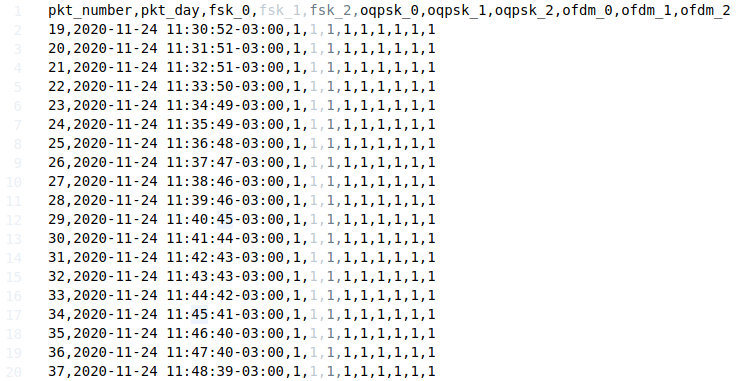
\includegraphics[width=\textwidth]{./sections/textual/chapters/images/second_csv_example.png}
            \label{fig:second_csv_example}
      \end{subfigure}
      \\Fonte: autoral.
      \label{fig:camposCSV}
\end{figure}

Todos os arquivos CSV e scripts utilizados para a análise de dados estão disponíveis no repositório \cite{wisun-traces}.

\section{Análise dos dados}

% \todo{falar sobre a largura de banda do canal OQPSK - afeta no PDR}\\
% \todo{Comparar o PDRxRSSI}\\
% \todo{Desvanecimento}

Os onze arquivos com as tentativas de transmissão foram computador e a partir disso foi calculado o PDR de cada modulação, estes valores são apresentados nas tabelas \ref{table:pdr1}, \ref{table:pdr2}, \ref{table:pdr3} e \ref{table:pdr4}, e apresentam os valores de PDR dos dispositivos agrupados por piso. Foi calculado também os valores de RSSI médios das transmissões recebidas, os valores, em dBm, são apresentados nas tabelas \ref{table:rssi1}, \ref{table:rssi2}, \ref{table:rssi3} e \ref{table:rssi4}.

\begin{table}
      \caption{Primeiro Piso}
      \begin{subtable}{\textwidth}
            \begin{center}
                  \begin{tabular}{|c|c|c|c|c|c|c|c|c|c|}
                        \hline
                        ID         & \multicolumn{3}{c|}{\textbf{SUN-FSK}} & \multicolumn{3}{c|}{\textbf{SUN-OQPSK}} & \multicolumn{3}{c|}{\textbf{SUN-OFDM}}                                                                                                       \\ \cline{2-10}
                                   & \textbf{P$_1$}                        & \textbf{P$_2$}                          & \textbf{P$_3$}                         & \textbf{P$_1$} & \textbf{P$_2$} & \textbf{P$_3$} & \textbf{P$_1$} & \textbf{P$_2$} & \textbf{P$_3$} \\ \hline
                        \texttt{D} & 80.39                                 & 78.71                                   & 80.17                                  & 99.20          & 99.17          & 99.17          & 99.21          & 99.21          & 99.21          \\ \hline
                        \texttt{H} & 80.86                                 & 78.67                                   & 80.97                                  & 99.21          & 99.21          & 99.21          & 45.12          & 45.19          & 45.31          \\ \hline
                  \end{tabular}
                  \caption{PDR}
                  \label{table:pdr1}
            \end{center}
      \end{subtable}%
      \\
      \par\bigskip
      \begin{subtable}{\textwidth}
            \begin{center}
                  \begin{tabular}{|c|c|c|c|c|c|c|c|c|c|}
                        \hline
                        ID         & \multicolumn{3}{c|}{\textbf{SUN-FSK}} & \multicolumn{3}{c|}{\textbf{SUN-OQPSK}} & \multicolumn{3}{c|}{\textbf{SUN-OFDM}}                                                                                                       \\ \cline{2-10}
                                   & \textbf{P$_1$}                        & \textbf{P$_2$}                          & \textbf{P$_3$}                         & \textbf{P$_1$} & \textbf{P$_2$} & \textbf{P$_3$} & \textbf{P$_1$} & \textbf{P$_2$} & \textbf{P$_3$} \\ \hline
                        \texttt{D} & -99.68                                & -99.52                                  & -99.62                                 & -90.39         & -90.42         & -90.38         & -98.54         & -98.20         & -98.67         \\ \hline
                        \texttt{H} & -106.05                               & -105.97                                 & -106.05                                & -90.75         & -90.78         & -90.76         & -108.36        & -108.37        & -108.19        \\ \hline
                  \end{tabular}
                  \caption{RSSI(dBm)}
                  \label{table:rssi1}
            \end{center}
      \end{subtable}%
      \label{tab:table1}
\end{table}

Importante destacar que os dispositivos Rx estavam no primeiro piso do prédio, o mesmo nível dos dispositivos ``D'' e ``H''. Mas os dispositivos Tx deste piso apresentam um menor desempenho a nível de aplicação (PDR) em relação aos dispositivos do segundo piso. Os valores de RSSI dos dispositivos presentes nos dois pisos não apresenta uma grande divergência, então, é deduzido que a diferença de valores de PDR é causada por áreas de sombreamento de sinal transmitido nos arredores dos receptores que levam a uma alta taxa de erros de \emph{bits} nas mensagens, tornando difícil o uso, por exemplo, de FEC, \emph{Forward Error Correction} (Códigos de Correção de Erros) o que leva a perda do pacote.

\begin{table}
      \caption{Segundo Piso}
      \begin{subtable}{\textwidth}
            \begin{center}
                  \begin{tabular}{|c|c|c|c|c|c|c|c|c|c|}
                        \hline
                        ID         & \multicolumn{3}{c|}{\textbf{SUN-FSK}} & \multicolumn{3}{c|}{\textbf{SUN-OQPSK}} & \multicolumn{3}{c|}{\textbf{SUN-OFDM}}                                                                                                       \\ \cline{2-10}
                                   & \textbf{P$_1$}                        & \textbf{P$_2$}                          & \textbf{P$_3$}                         & \textbf{P$_1$} & \textbf{P$_2$} & \textbf{P$_3$} & \textbf{P$_1$} & \textbf{P$_2$} & \textbf{P$_3$} \\ \hline
                        \texttt{A} & 99.17                                 & 99.15                                   & 99.15                                  & 99.20          & 99.21          & 99.21          & 99.15          & 99.15          & 99.18          \\ \hline
                        \texttt{B} & 98.08                                 & 97.93                                   & 98.10                                  & 97.85          & 98.32          & 98.44          & 99.04          & 98.94          & 99.02          \\ \hline
                        \texttt{C} & 28.11                                 & 20.21                                   & 28.17                                  & 99.07          & 98.95          & 99.01          & 96.40          & 96.40          & 96.37          \\ \hline
                  \end{tabular}
                  \caption{PDR}
                  \label{table:pdr2}
            \end{center}
      \end{subtable}%
      \\
      \par\bigskip
      \begin{subtable}{\textwidth}
            \begin{center}
                  \begin{tabular}{|c|c|c|c|c|c|c|c|c|c|}
                        \hline
                        ID         & \multicolumn{3}{c|}{\textbf{SUN-FSK}} & \multicolumn{3}{c|}{\textbf{SUN-OQPSK}} & \multicolumn{3}{c|}{\textbf{SUN-OFDM}}                                                                                                       \\ \cline{2-10}
                                   & \textbf{P$_1$}                        & \textbf{P$_2$}                          & \textbf{P$_3$}                         & \textbf{P$_1$} & \textbf{P$_2$} & \textbf{P$_3$} & \textbf{P$_1$} & \textbf{P$_2$} & \textbf{P$_3$} \\ \hline
                        \texttt{A} & -98.31                                & -98.29                                  & -98.30                                 & -81.76         & -81.76         & -81.76         & -103.01        & -103.18        & -103.01        \\ \hline
                        \texttt{B} & -100.27                               & -100.26                                 & -100.28                                & -88.96         & -89.13         & -89.15         & -101.32        & -101.36        & -101.11        \\ \hline
                        \texttt{C} & -109.06                               & -108.67                                 & -109.07                                & -91.13         & -91.14         & -91.11         & -106.81        & -106.88        & -106.68        \\ \hline
                  \end{tabular}
                  \caption{RSSI(dBm)}
                  \label{table:rssi2}
            \end{center}
      \end{subtable}%
      \label{tab:table1}
\end{table}

\begin{table}
      \caption{Terceiro Piso}
      \begin{subtable}{\textwidth}
            \begin{center}
                  \begin{tabular}{|c|c|c|c|c|c|c|c|c|c|}
                        \hline
                        ID         & \multicolumn{3}{c|}{\textbf{SUN-FSK}} & \multicolumn{3}{c|}{\textbf{SUN-OQPSK}} & \multicolumn{3}{c|}{\textbf{SUN-OFDM}}                                                                                                       \\ \cline{2-10}
                                   & \textbf{P$_1$}                        & \textbf{P$_2$}                          & \textbf{P$_3$}                         & \textbf{P$_1$} & \textbf{P$_2$} & \textbf{P$_3$} & \textbf{P$_1$} & \textbf{P$_2$} & \textbf{P$_3$} \\ \hline
                        \texttt{E} & 69.71                                 & 63.88                                   & 69.71                                  & 99.20          & 99.21          & 99.21          & 98.53          & 98.60          & 98.58          \\ \hline
                        \texttt{F} & 86.56                                 & 83.35                                   & 85.67                                  & 99.21          & 99.21          & 99.18          & 88.12          & 88.23          & 88.17          \\ \hline
                        \texttt{G} & 0.18                                  & 0.15                                    & 0.15                                   & 76.59          & 76.45          & 75.82          & 0.07           & 0.07           & 0.15           \\ \hline
                  \end{tabular}
                  \caption{PDR}
                  \label{table:pdr3}
            \end{center}
      \end{subtable}%
      \\
      \par\bigskip
      \begin{subtable}{\textwidth}
            \begin{center}
                  \begin{tabular}{|c|c|c|c|c|c|c|c|c|c|}
                        \hline
                        ID         & \multicolumn{3}{c|}{\textbf{SUN-FSK}} & \multicolumn{3}{c|}{\textbf{SUN-OQPSK}} & \multicolumn{3}{c|}{\textbf{SUN-OFDM}}                                                                                                       \\ \cline{2-10}
                                   & \textbf{P$_1$}                        & \textbf{P$_2$}                          & \textbf{P$_3$}                         & \textbf{P$_1$} & \textbf{P$_2$} & \textbf{P$_3$} & \textbf{P$_1$} & \textbf{P$_2$} & \textbf{P$_3$} \\ \hline

                        \texttt{E} & -105.77                               & -105.65                                 & -105.74                                & -86.88         & -86.89         & -86.88         & -106.06        & -106.13        & -105.92        \\ \hline
                        \texttt{F} & -104.92                               & -104.83                                 & -104.90                                & -86.23         & -86.26         & -86.22         & -108.02        & -108.01        & -107.87        \\ \hline
                        \texttt{G} & -111.42                               & -111.50                                 & -111.70                                & -104.36        & -104.38        & -104.32        & -112.80        & -112.80        & -112.80        \\ \hline
                  \end{tabular}
                  \caption{RSSI(dBm)}
                  \label{table:rssi3}
            \end{center}
      \end{subtable}%
      \label{tab:table1}
\end{table}

Os dados obtidos dos dispositivos presentes no quarto piso do prédio mostram que o dispositivo ``K'' obteve PDR entre 97\% e 99\% nas modulações SUN-OQPSK e SUN-FSK e cerca de 56\% na modulação SUN-OFDM. A disparidade de valores entre este dispositivo e os outros do mesmo piso é atribuído, principalmente, ao fato de que o dispositivo encontra-se em uma sala diretamente acima da sala dos dispositivos Rx.

O motivo da modulação SUN-OFDM obter um pior desempenho, nos valores de PDR, em relação as outras modulações no dispositivo ``K'' é atribuída ao desvanecimento do sinal já que, de acordo com a Tabela \ref{table:config}, a modulação possui o menor valor de potência de transmissão das três modulações.

\begin{table}
      \caption{Quarto Piso}
      \begin{subtable}{\textwidth}
            \begin{center}
                  \begin{tabular}{|c|c|c|c|c|c|c|c|c|c|}
                        \hline
                        ID         & \multicolumn{3}{c|}{\textbf{SUN-FSK}} & \multicolumn{3}{c|}{\textbf{SUN-OQPSK}} & \multicolumn{3}{c|}{\textbf{SUN-OFDM}}                                                                                                       \\ \cline{2-10}
                                   & \textbf{P$_1$}                        & \textbf{P$_2$}                          & \textbf{P$_3$}                         & \textbf{P$_1$} & \textbf{P$_2$} & \textbf{P$_3$} & \textbf{P$_1$} & \textbf{P$_2$} & \textbf{P$_3$} \\ \hline

                        \texttt{I} & 6.10                                  & 5.77                                    & 6.12                                   & 57.90          & 57.92          & 58.36          & 0.00           & 0.00           & 0.00           \\ \hline
                        \texttt{J} & 0.01                                  & 0.01                                    & 0.00                                   & 25.02          & 25.33          & 24.86          & 1.78           & 1.94           & 1.83           \\ \hline
                        \texttt{K} & 97.56                                 & 97.36                                   & 97.53                                  & 98.15          & 98.15          & 98.16          & 56.75          & 57.29          & 56.89          \\ \hline
                  \end{tabular}
                  \caption{PDR}
                  \label{table:pdr4}
            \end{center}
      \end{subtable}%
      \\
      \par\bigskip
      \begin{subtable}{\textwidth}
            \begin{center}
                  \begin{tabular}{|c|c|c|c|c|c|c|c|c|c|}
                        \hline
                        ID         & \multicolumn{3}{c|}{\textbf{SUN-FSK}} & \multicolumn{3}{c|}{\textbf{SUN-OQPSK}} & \multicolumn{3}{c|}{\textbf{SUN-OFDM}}                                                                                                       \\ \cline{2-10}
                                   & \textbf{P$_1$}                        & \textbf{P$_2$}                          & \textbf{P$_3$}                         & \textbf{P$_1$} & \textbf{P$_2$} & \textbf{P$_3$} & \textbf{P$_1$} & \textbf{P$_2$} & \textbf{P$_3$} \\ \hline

                        \texttt{I} & -112.21                               & -112.20                                 & -112.18                                & -105.09        & -105.11        & -105.10        & N/A            & N/A            & N/A            \\ \hline
                        \texttt{J} & -112.00                               & -113.00                                 & N/A                                    & -106.62        & -106.68        & -106.59        & -112.56        & -112.56        & -112.54        \\ \hline
                        \texttt{K} & -101.33                               & -101.30                                 & -101.33                                & -90.29         & -90.34         & -90.32         & -109.19        & -109.26        & -109.16        \\ \hline
                  \end{tabular}
                  \caption{RSSI(dBm)}
                  \label{table:rssi4}
            \end{center}
      \end{subtable}%
      \label{tab:table1}
\end{table}


% \begin{table}[ht]
%       \centering
%       \caption{Valores de PDR para cada dispositivo.}
%       \begin{tabular}{|c|c|c|c|c|c|c|c|c|c|}
%             \hline
%             ID                     & \multicolumn{3}{c|}{\textbf{SUN-FSK}} & \multicolumn{3}{c|}{\textbf{SUN-OQPSK}} & \multicolumn{3}{c|}{\textbf{SUN-OFDM}}                                                                                                       \\ \cline{2-10}
%                                    & \textbf{P$_1$}                        & \textbf{P$_2$}                          & \textbf{P$_3$}                         & \textbf{P$_1$} & \textbf{P$_2$} & \textbf{P$_3$} & \textbf{P$_1$} & \textbf{P$_2$} & \textbf{P$_3$} \\ \hline
%             \texttt{D}             & 80.39                                 & 78.71                                   & 80.17                                  & 99.20          & 99.17          & 99.17          & 99.21          & 99.21          & 99.21          \\ \hline
%             \texttt{H}             & 80.86                                 & 78.67                                   & 80.97                                  & 99.21          & 99.21          & 99.21          & 45.12          & 45.19          & 45.31          \\ \hline
% \texttt{A}             & 99.17                                 & 99.15                                   & 99.15                                  & 99.20          & 99.21          & 99.21          & 99.15          & 99.15          & 99.18          \\ \hline
% \texttt{B}             & 98.08                                 & 97.93                                   & 98.10                                  & 97.85          & 98.32          & 98.44          & 99.04          & 98.94          & 99.02          \\ \hline
% \texttt{C}             & 28.11                                 & 20.21                                   & 28.17                                  & 99.07          & 98.95          & 99.01          & 96.40          & 96.40          & 96.37          \\ \hline
% \texttt{E}             & 69.71                                 & 63.88                                   & 69.71                                  & 99.20          & 99.21          & 99.21          & 98.53          & 98.60          & 98.58          \\ \hline
% \texttt{F}             & 86.56                                 & 83.35                                   & 85.67                                  & 99.21          & 99.21          & 99.18          & 88.12          & 88.23          & 88.17          \\ \hline
% \texttt{G}             & 0.18                                  & 0.15                                    & 0.15                                   & 76.59          & 76.45          & 75.82          & 0.07           & 0.07           & 0.15           \\ \hline
%             \texttt{I}             & 6.10                                  & 5.77                                    & 6.12                                   & 57.90          & 57.92          & 58.36          & 0.00           & 0.00           & 0.00           \\ \hline
%             \texttt{J}             & 0.01                                  & 0.01                                    & 0.00                                   & 25.02          & 25.33          & 24.86          & 1.78           & 1.94           & 1.83           \\ \hline
%             \texttt{K}             & 97.56                                 & 97.36                                   & 97.53                                  & 98.15          & 98.15          & 98.16          & 56.75          & 57.29          & 56.89          \\ \hline
%             \textbf{Média}         & 58.79                                 & 56.83                                   & 58.70                                  & 86.42          & 86.47          & 86.42          & 62.20          & 62.28          & 62.25          \\ \hline
%             \textbf{Desvio Padrão} & 41.39                                 & 41.50                                   & 41.32                                  & 24.34          & 24.28          & 24.39          & 43.54          & 43.51          & 43.52          \\ \hline
%       \end{tabular}
%       \label{table:pdr}
% \end{table}

% \begin{table}[ht]
%       \centering
%       \caption{Valores de PDR para cada dispositivo.}
%       \begin{tabular}{|c|c|c|c|c|c|c|c|c|c|}
%             \hline
%             ID         & \multicolumn{3}{c|}{\textbf{SUN-FSK}} & \multicolumn{3}{c|}{\textbf{SUN-OQPSK}} & \multicolumn{3}{c|}{\textbf{SUN-OFDM}}                                                                                                       \\ \cline{2-10}
%                        & \textbf{P$_1$}                        & \textbf{P$_2$}                          & \textbf{P$_3$}                         & \textbf{P$_1$} & \textbf{P$_2$} & \textbf{P$_3$} & \textbf{P$_1$} & \textbf{P$_2$} & \textbf{P$_3$} \\ \hline
%             \texttt{D} & -99.68                                & -99.52                                  & -99.62                                 & -90.39         & -90.42         & -90.38         & -98.54         & -98.20         & -98.67         \\ \hline
%             \texttt{H} & -106.05                               & -105.97                                 & -106.05                                & -90.75         & -90.78         & -90.76         & -108.36        & -108.37        & -108.19        \\ \hline
% \texttt{A} & -98.31                                & -98.29                                  & -98.30                                 & -81.76         & -81.76         & -81.76         & -103.01        & -103.18        & -103.01        \\ \hline
% \texttt{B} & -100.27                               & -100.26                                 & -100.28                                & -88.96         & -89.13         & -89.15         & -101.32        & -101.36        & -101.11        \\ \hline
% \texttt{C} & -109.06                               & -108.67                                 & -109.07                                & -91.13         & -91.14         & -91.11         & -106.81        & -106.88        & -106.68        \\ \hline
% \texttt{E} & -105.77                               & -105.65                                 & -105.74                                & -86.88         & -86.89         & -86.88         & -106.06        & -106.13        & -105.92        \\ \hline
% \texttt{F} & -104.92                               & -104.83                                 & -104.90                                & -86.23         & -86.26         & -86.22         & -108.02        & -108.01        & -107.87        \\ \hline
% \texttt{G} & -111.42                               & -111.50                                 & -111.70                                & -104.36        & -104.38        & -104.32        & -112.80        & -112.80        & -112.80        \\ \hline
% \texttt{I} & -112.21                               & -112.20                                 & -112.18                                & -105.09        & -105.11        & -105.10        & N/A            & N/A            & N/A            \\ \hline
% \texttt{J} & -112.00                               & -113.00                                 & N/A                                    & -106.62        & -106.68        & -106.59        & -112.56        & -112.56        & -112.54        \\ \hline
% \texttt{K} & -101.33                               & -101.30                                 & -101.33                                & -90.29         & -90.34         & -90.32         & -109.19        & -109.26        & -109.16        \\ \hline
%             % \textbf{Média} & -105.55                               & -105.56                                 & -95.38                                 & -92.95         & -92.99         & -92.96         & -96.97         & -96.98         & -96.90         \\ \hline
%             % \makecell{\textbf{Desvio}                                                                                                                                                                                                                       \\\textbf{Padrão}} & 5.16                                  & 5.30                                    & 31.99                                  & 8.42           & 8.42           & 8.41           & 32.46          & 32.47          & 32.44          \\ \hline
%       \end{tabular}
%       \label{table:rssi}
% \end{table}

% D = -99.68 & -99.52 & -99.62 & -90.39 & -90.42 & -90.38 & -98.54 & -98.20 & -98.67
% H = -106.05 & -105.97 & -106.05 & -90.75 & -90.78 & -90.76 & -108.36 & -108.37 & -108.19
% A = -98.31 & -98.29 & -98.30 & -81.76 & -81.76 & -81.76 & -103.01 & -103.18 & -103.01
% B = -100.27 & -100.26 & -100.28 & -88.96 & -89.13 & -89.15 & -101.32 & -101.36 & -101.11
% C = -109.06 & -108.67 & -109.07 & -91.13 & -91.14 & -91.11 & -106.81 & -106.88 & -106.68
% E = -105.77 & -105.65 & -105.74 & -86.88 & -86.89 & -86.88 & -106.06 & -106.13 & -105.92
% F = -104.92 & -104.83 & -104.90 & -86.23 & -86.26 & -86.22 & -108.02 & -108.01 & -107.87
% G = -111.42 & -111.50 & -111.70 & -104.36 & -104.38 & -104.32 & -112.80 & -112.80 & -112.80
% I = -112.21 & -112.20 & -112.18 & -105.09 & -105.11 & -105.10 & -0.00 & -0.00 & -0.00
% J = -112.00 & -113.00 & -0.00 & -106.62 & -106.68 & -106.59 & -112.56 & -112.56 & -112.54
% K = -101.33 & -101.30 & -101.33 & -90.29 & -90.34 & -90.32 & -109.19 & -109.26 & -109.16

Os gráficos apresentados na Figura \ref{fig:pdr_andar}, mostram a média dos valores de PDR por piso de acordo com as modulações e o ciclo de transmissão. \refact{A linha preta} mostra os valores mínimos e máximos de PDR do piso.

Observando os gráficos da Figura \ref{fig:pdr_andar}, a modulação SUN-OQPSK se destaca em relação às outras. Como apresentado na Seção \ref{padrõesSF}, as modulações SUN-OQPSK e SUN-OFDM apresentam maior robustez a interferências e efeitos negativos da propagação por múltiplos caminhos. Porém, como apresentado na Tabela \ref{table:config}, a modulação SUN-OQPSK apresenta maior potência de transmissão e maior largura de banda do canal, o que garante, junto com a técnica de modulação do DSSS-OQPSK, Seção \ref{oqpsk}, melhor aproveitamento do canal de transmissão e, consequentemente, uma melhor recepção do sinal.

\begin{figure}[ht!]
      \centering
      \caption{Valores de PDR para cada piso.}
      \begin{subfigure}{.4\textwidth}
            \centering
            \caption{Primeiro Piso.}
            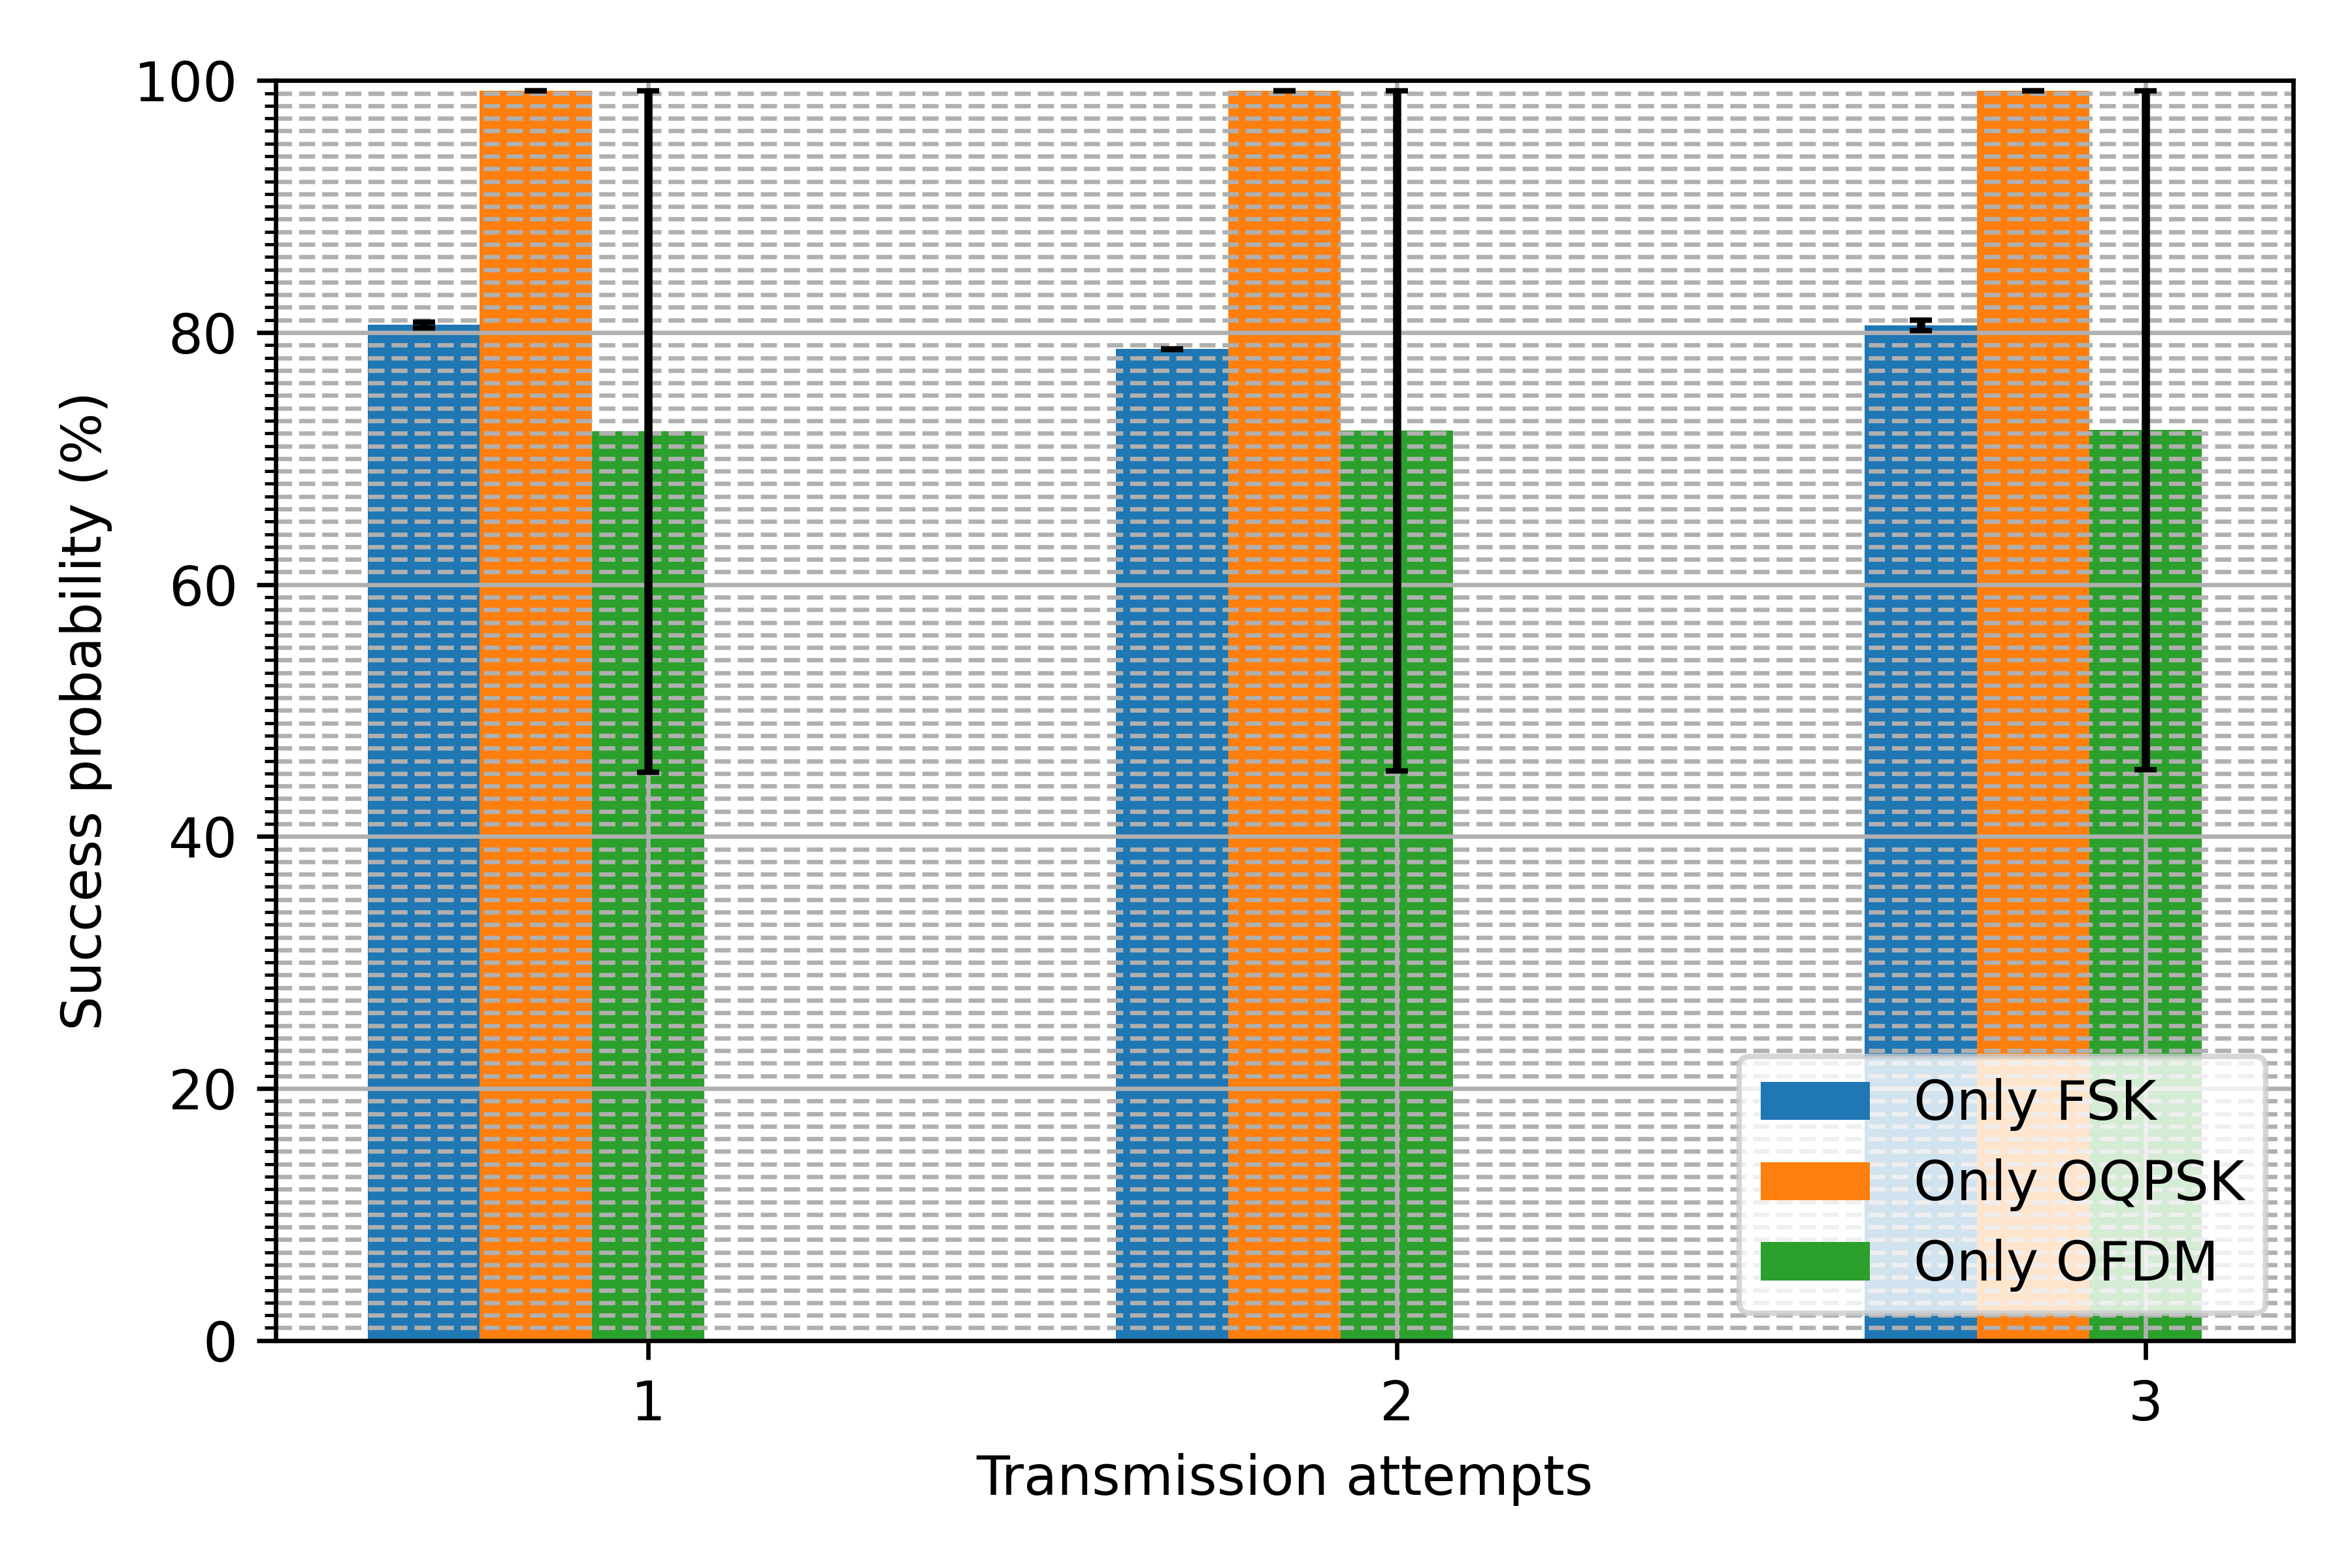
\includegraphics[width=\textwidth]{./sections/textual/chapters/images/mod_1_floor.png}
            \label{fig:piso1}
      \end{subfigure}
      \begin{subfigure}{.4\textwidth}
            \centering
            \caption{Segundo Piso.}
            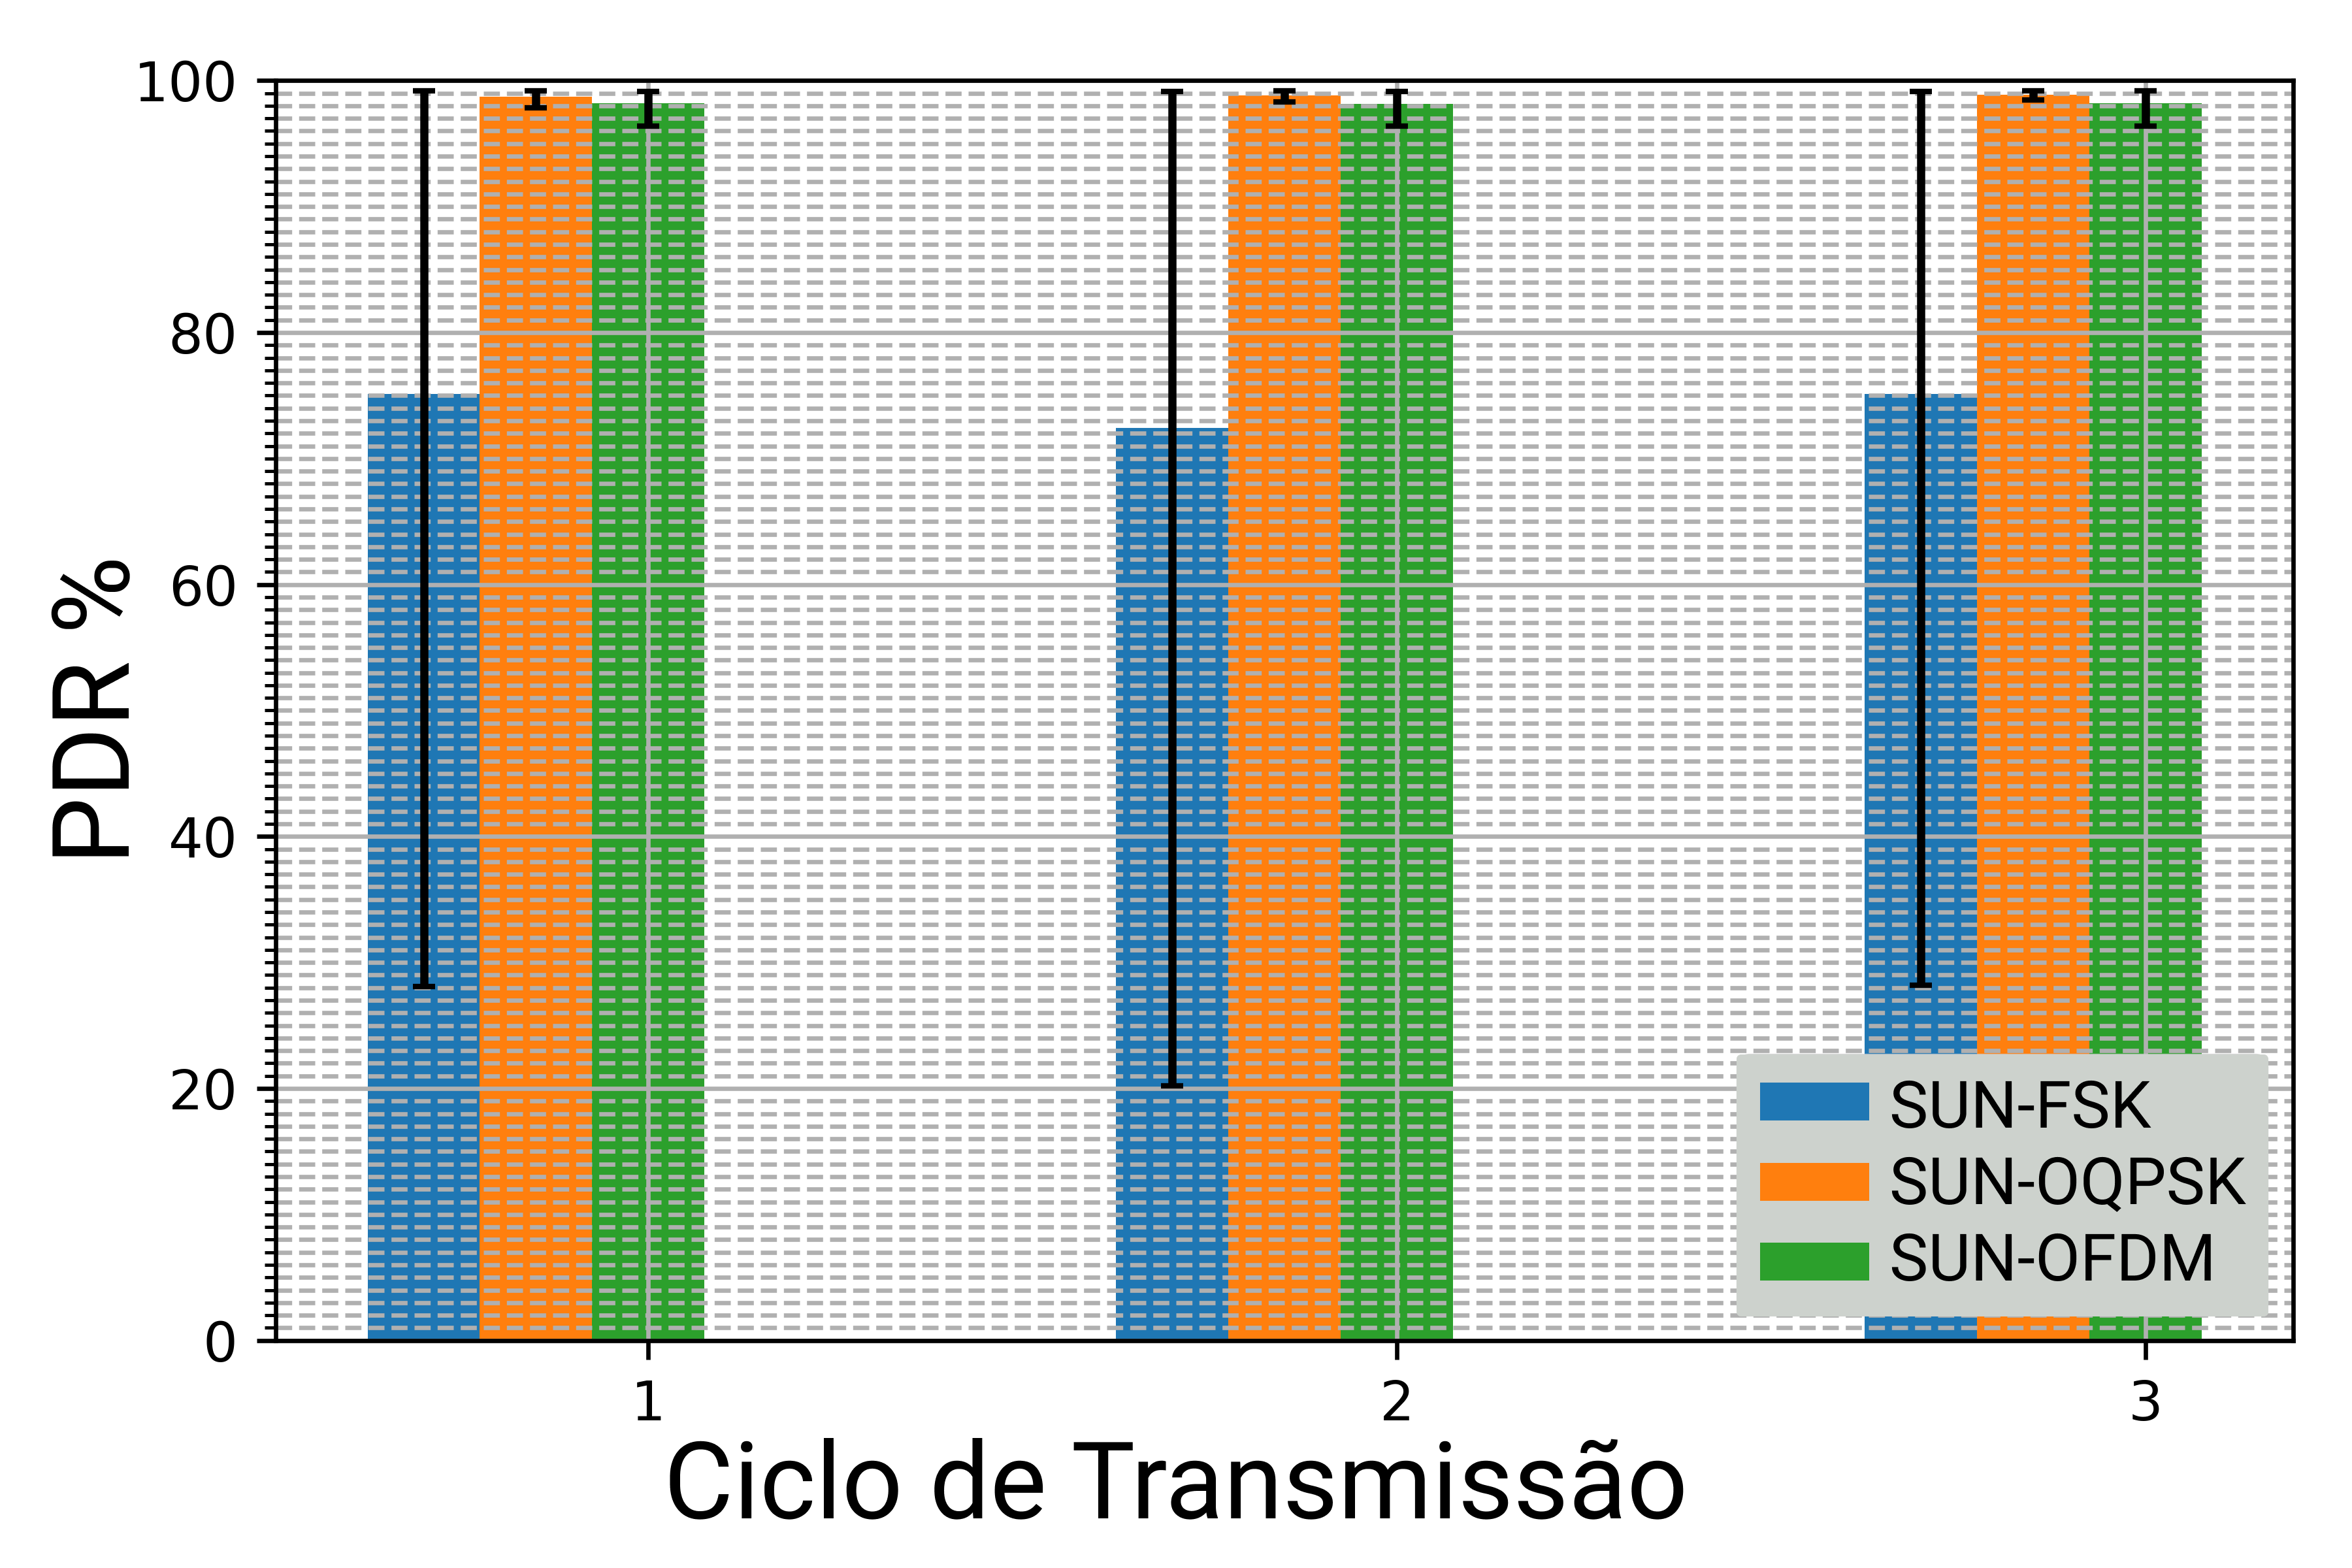
\includegraphics[width=\textwidth]{./sections/textual/chapters/images/mod_2_floor.png}
            \label{fig:piso2}
      \end{subfigure}
      \begin{subfigure}{.4\textwidth}
            \centering
            \caption{Terceiro Piso.}
            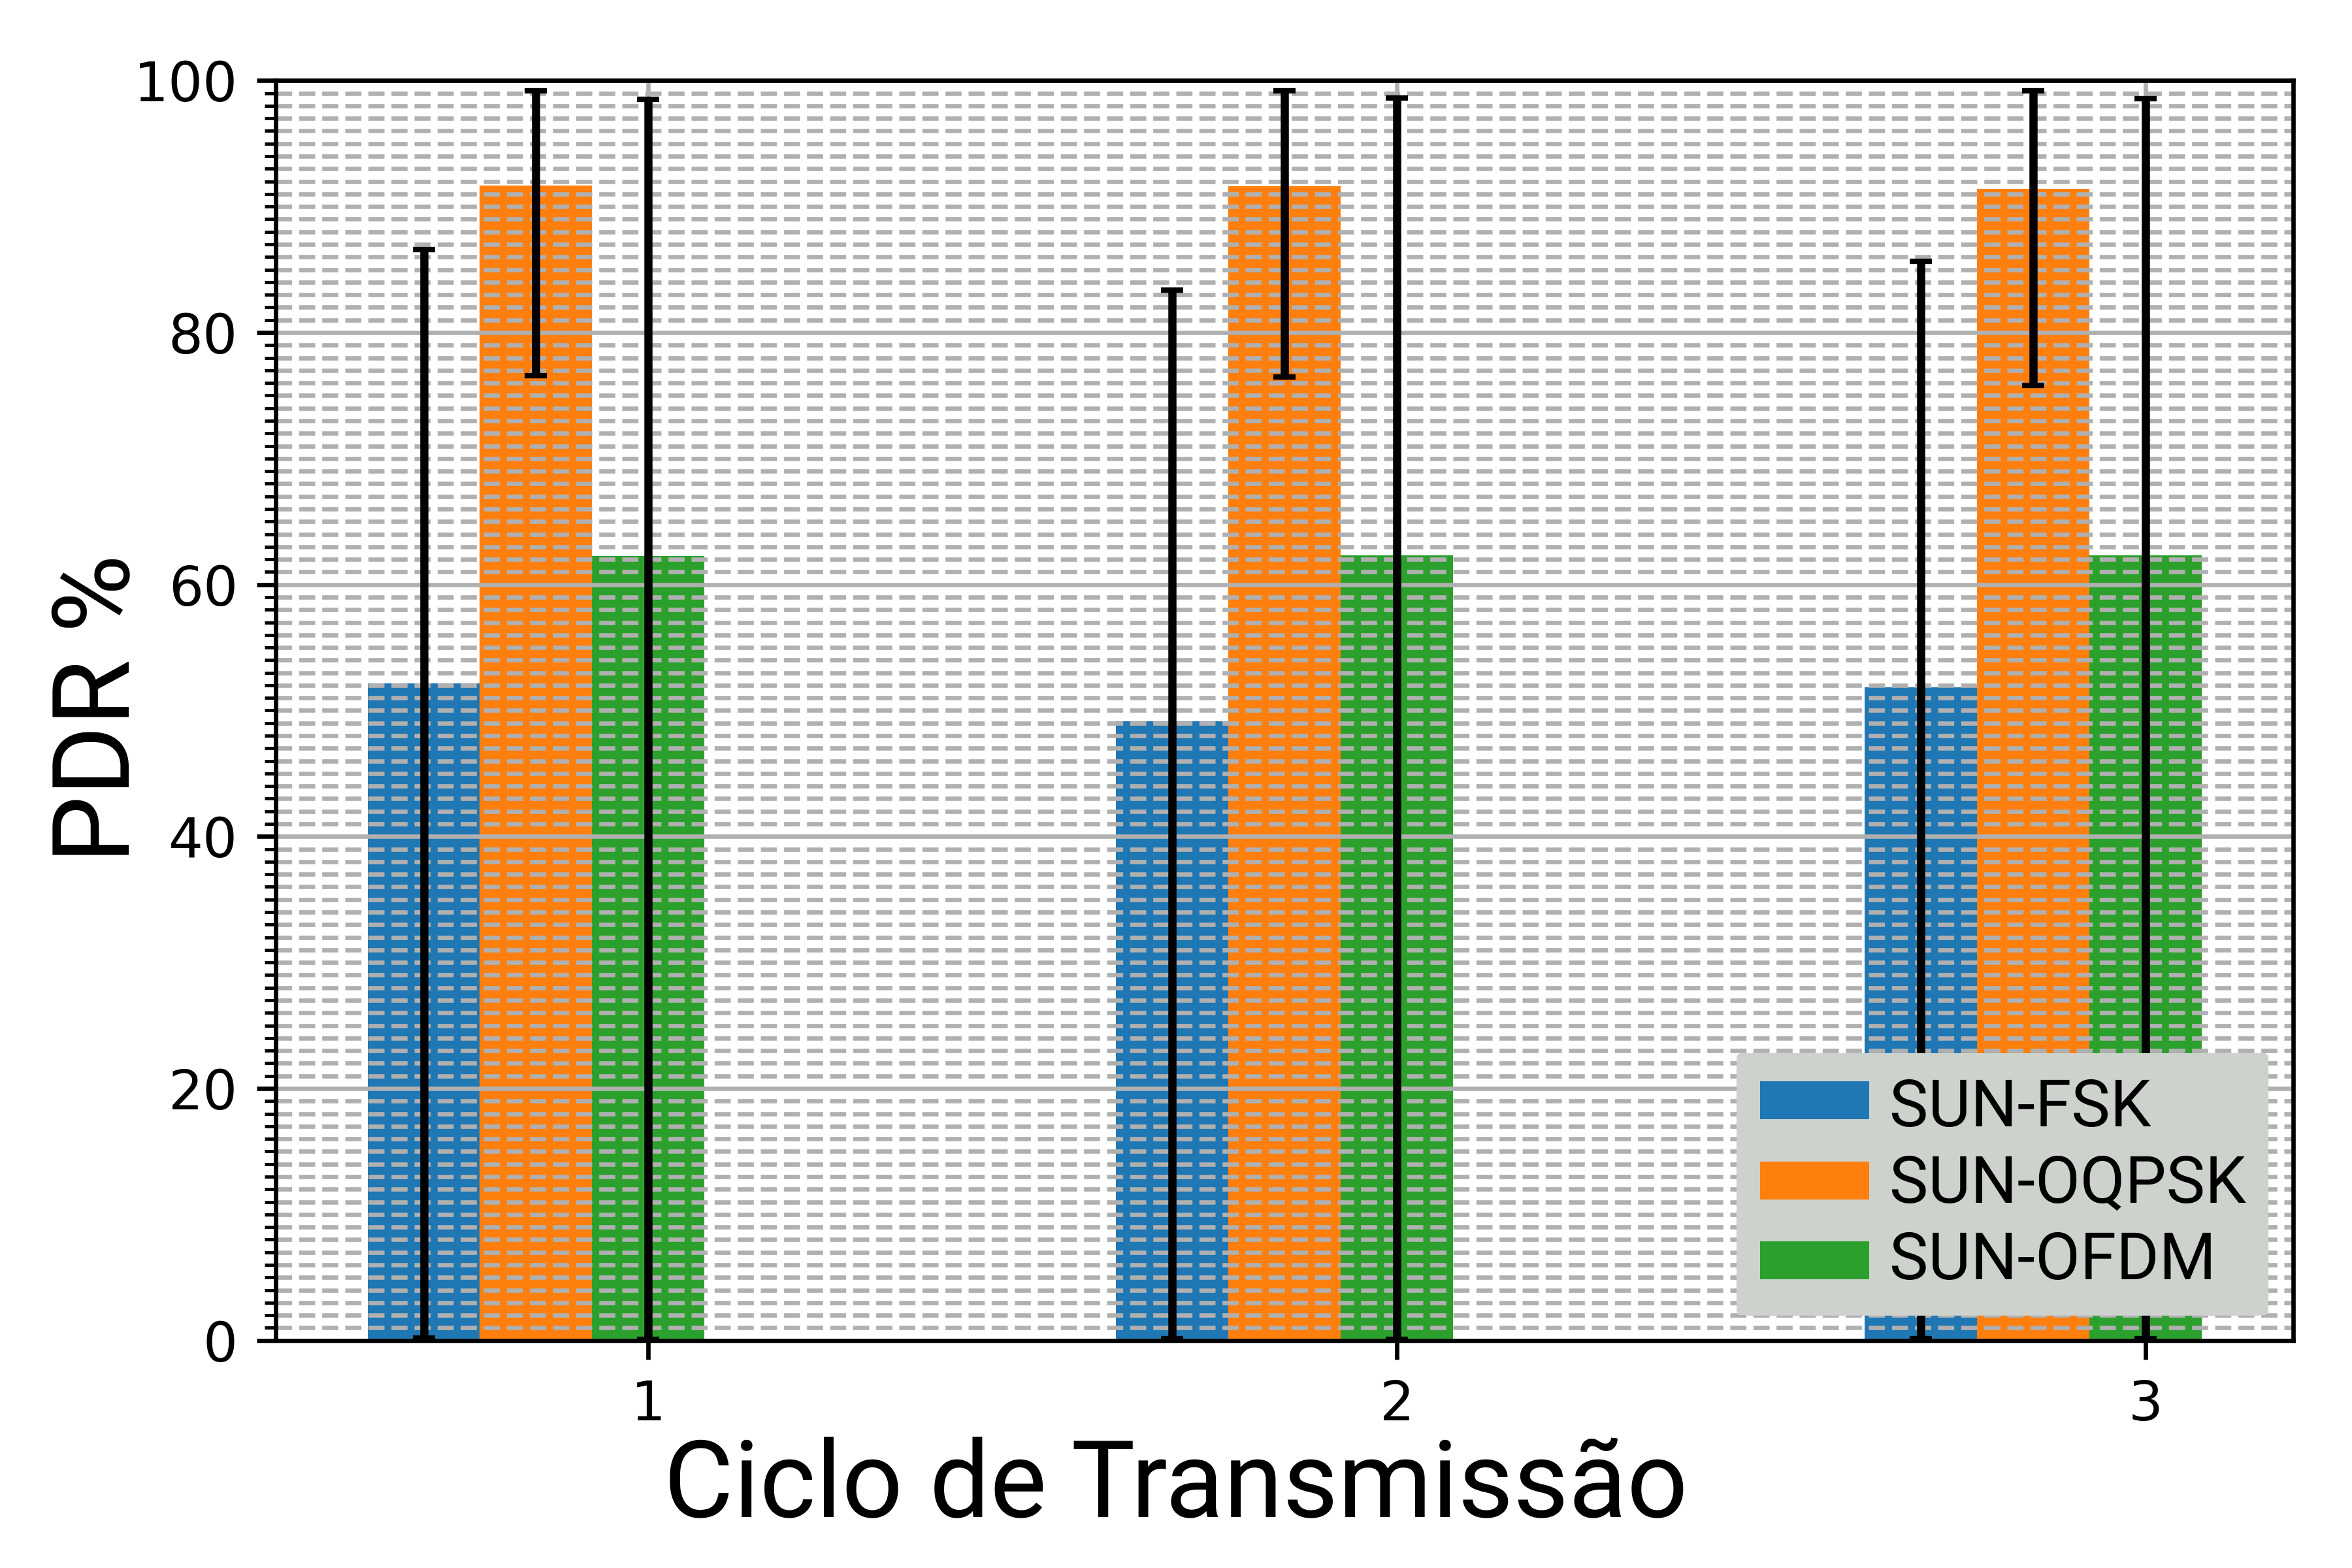
\includegraphics[width=\textwidth]{./sections/textual/chapters/images/mod_3_floor.png}
            \label{fig:piso3}
      \end{subfigure}
      \begin{subfigure}{.4\textwidth}
            \centering
            \caption{Quarto Piso.}
            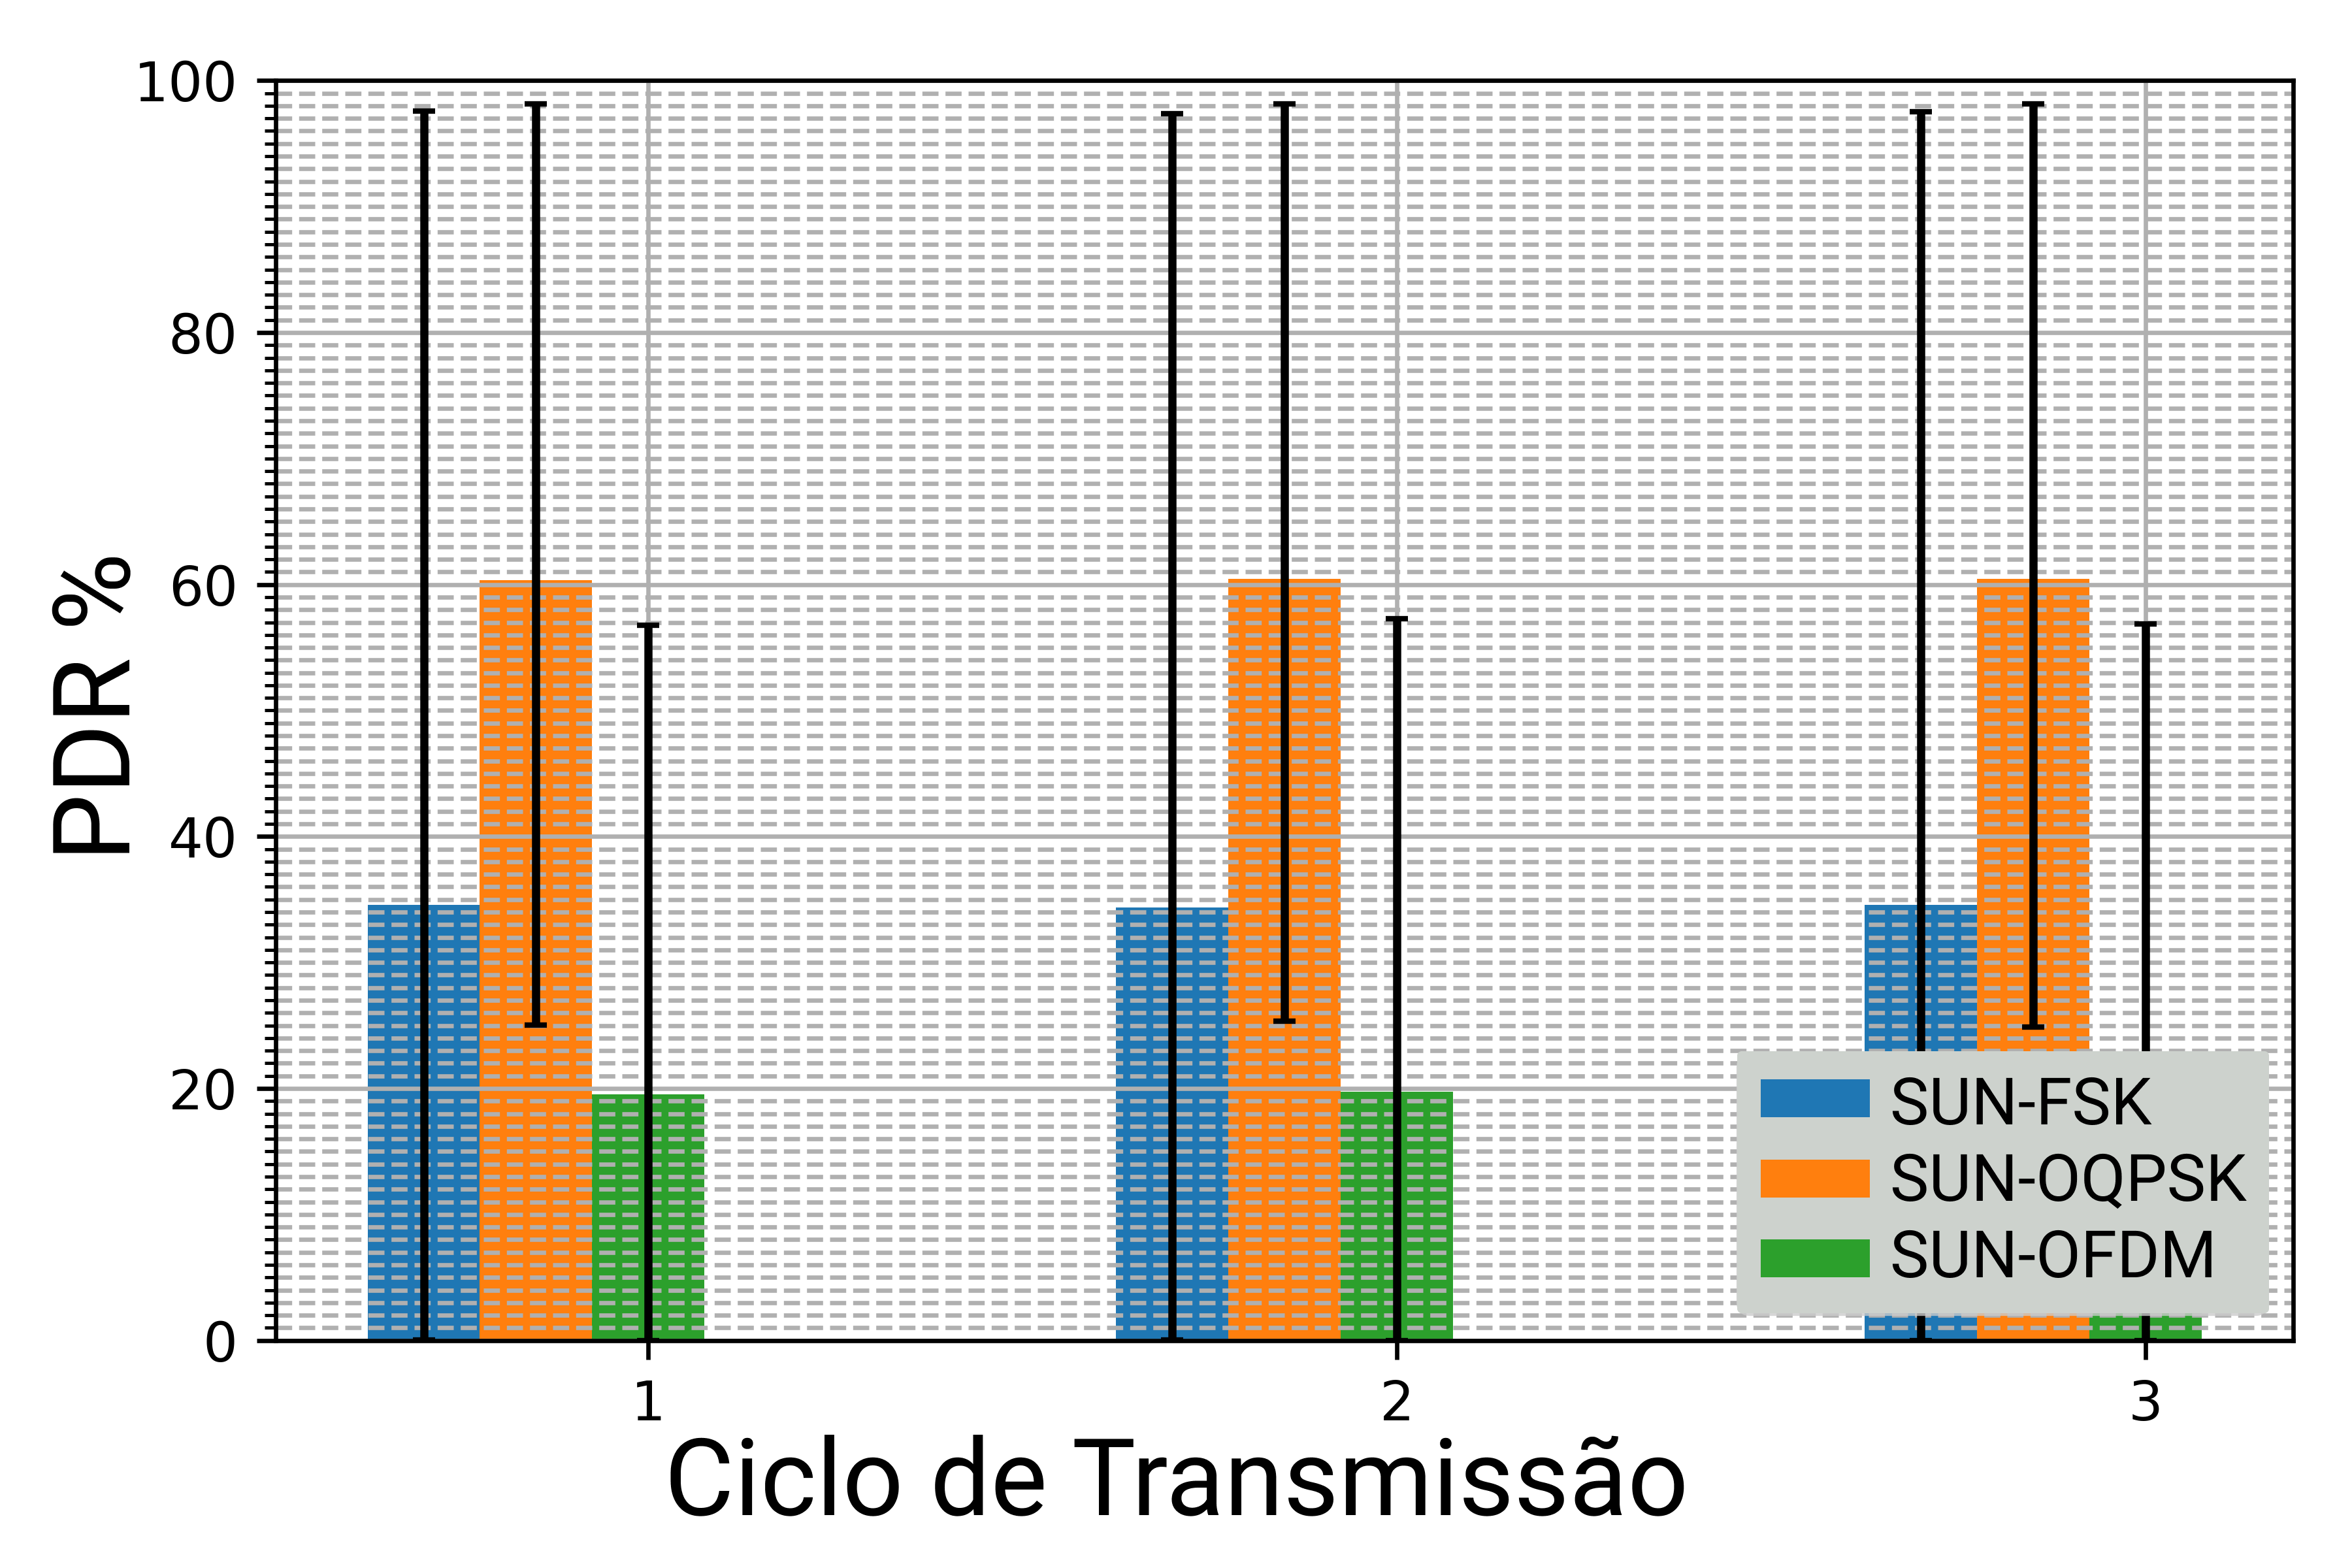
\includegraphics[width=\textwidth]{./sections/textual/chapters/images/mod_4_floor.png}
            \label{fig:piso4}
      \end{subfigure}
      \label{fig:pdr_andar}
\end{figure}


% \todo{Fazer a analise de RSSI e CCA}


